\documentclass[14pt]{article}
\usepackage[T2A]{fontenc} 
\usepackage[utf8]{inputenc}
\usepackage{alltt}
\usepackage[english,russian]{babel}
\usepackage{amsmath}
\usepackage{amsfonts}
\usepackage{amssymb}
\usepackage{wrapfig}
\usepackage{indentfirst}
\usepackage{setspace}
\usepackage[pdftex]{graphicx}
\usepackage{caption}
\usepackage{subcaption}
\usepackage{textcomp}
\usepackage{array}


\topmargin = -1.5cm
\marginparwidth = -1cm
\marginparsep = 0pt
\textwidth = 16cm
\textheight = 24cm
\oddsidemargin = 0.2cm
\parindent = 0.5cm
\lineskip = 0.025cm
\parskip = 0.2cm




\begin{document}

\begin{titlepage}

\newcommand{\HRule}{\rule{\linewidth}{0.5mm}} 
\centering 

\begin{figure}
    \centering
    \begin{subfigure}{1.5cm}
       
\includegraphics[height=1.3cm]{msu.jpg}
    \end{subfigure}
    \parbox[t][0.2cm][c]{12cm}{
        \centering
        \large Московский государственный университет имени М.~В.~Ломоносова\\[0.5cm]
        \normalsize Факультет вычислительной математики и кибернетики
    }
    \begin{subfigure}{1.25cm}    
        
\includegraphics[height=1.25cm]{cmc.jpg}
    \end{subfigure}
\end{figure}



\HRule \\[5cm]
{
 \bfseries \upshape
{ \Huge  \guillemotleftРекурсивные нейросети с памятью\guillemotright }\\[0.2cm]
{\LARGE Реферат}\\[0.2cm]

{
\large
\vspace{1cm}
студента $203$ учебной группы факультета ВМК МГУ \\
Щербакова Александра Станиславовича
}

\vspace{9cm}
{\large Москва, \today}
} 


\vfill

\end{titlepage}

\tableofcontents
\pagebreak
\section{Введение}

\large
Рекурсивные нейронные сети (Recursive Neural Networks, RNN) известны уже около 20-ти лет. Это вид глубоких нейронных сетей, которые работают с некоторым набором весов рекурсивно. Рекурсивные нейросети используются для обработки естественных языков, работы с последовательностями, изображениями.


\section{Рекурсивные нейросети}

\subsection{Описание}
\largeРекурсивные нейронные сети подходят для задачи классификации и регрессии. Они широко используются в моделях с информацией в числовом и символьном виде. Важным преимуществом рекурсивных нейросетей является их возможность работать с информацией имеющей топологию отличную от вектора фиксированного размера. Таким образом для информации, представленной в виде графа, сохраняются связи между вершинами графа. Но есть существенное ограничение на топологию графов, с которыми ведет работу нейронная сеть этого типа - они должны быть ацикличны. Это связано с тем, что ребра графа интерпретируются как причинно-следственная связь. Есть примеры рекурсивных нейронных сетей, которые обрабатывают циклические графы, но они, как правило, могут быть использованы только в очень редких конкретных видах задач.


Второе ограничение связано с достаточно слабым математическим аппаратом такой сети. В частности, отсутствие такой операции как сумма графов.


В качестве алгоритма для обучения рекурсивной нейронной сети можно использовать алгоритм стохастического градиентного спуска второго порядка. Этот метод устойчив к затуханию градиента. Так же он обеспечивает оптимальный компромисс между скоростью сходимости и вычислительносй сложностью вычислений.


Можно провести параллель между такой сетью и интеллектом. У интеллекта есть два основопологающий принципа: максимизация передачи и принцип возвратности. Первый из них гласит, что всегда, когда это возможно интеллектуальная система накапливает знания путем максимизации передачи полученных ранее знаний. Таким образом система становится более сложной накапливая все новые знания. Принцип возвратности связывает память и логические выводы. Он утверждает, что система является интеллектуальной, если она может восстановить причины своего состояния.

\subsection{Структура}
\largeПусть дан граф $U = (V, E)$. Для вершины $v\in V$ $pa[v]$ - множество вершин родителей, $ch[v]$ - множество  дочерних вершин. Под родительской вершиной будем подразумевать ту, в которую ведет ребро из $v$, а под дочерней - вершину, из которой есть ребро в $v$. Этот граф будет описывать единицы информации, с которыми работает нейросеть. В каждой вершине содержится фрагмент информации, а налачие ребра между двумя вершинами подразумевает их связь.


Модель рекурсивной нейронной сети включает в себя функцию изменения состояния $f$ и выходную функцию $g$. Обычно эти функции реализуются многослойным перцептроном. Стандартная модель подходит для обработки направленных ациклических графов с одним корнем. Они реализуют пересчет состояния сети с учетом предыдущего шага:


\begin{eqnarray}
&a(v) = f(a(ch[v]), I(v), v, W_f)\nonumber\\
&y(v) = g(a(v), v, W_g)
\end{eqnarray}


Где $W_f$ и $W_g$ - матрицы синаптических весов для сетей $f$ и $g$. Это параметры модели. $a(v)$ - состояние вершины. Для каждой вершины состояние пересчитывается из входного сигнала $I(v)$ и состояний дочерних вершин $ch[v]$.


\begin{equation}
\label{trivial}
a(ch[v]) = [a(ch_1[v]), a(ch_2[v]), \dots, a(ch_o[v])]
\end{equation}


В выражении $(2)$ $o$ - максимальное количество дочерних элементов. Результат работы нейронной сети (вывод вершины-корня $s$) вычисляется по формуле $y = g(a(s))$.


\begin{figure}[!h]
    \centering
        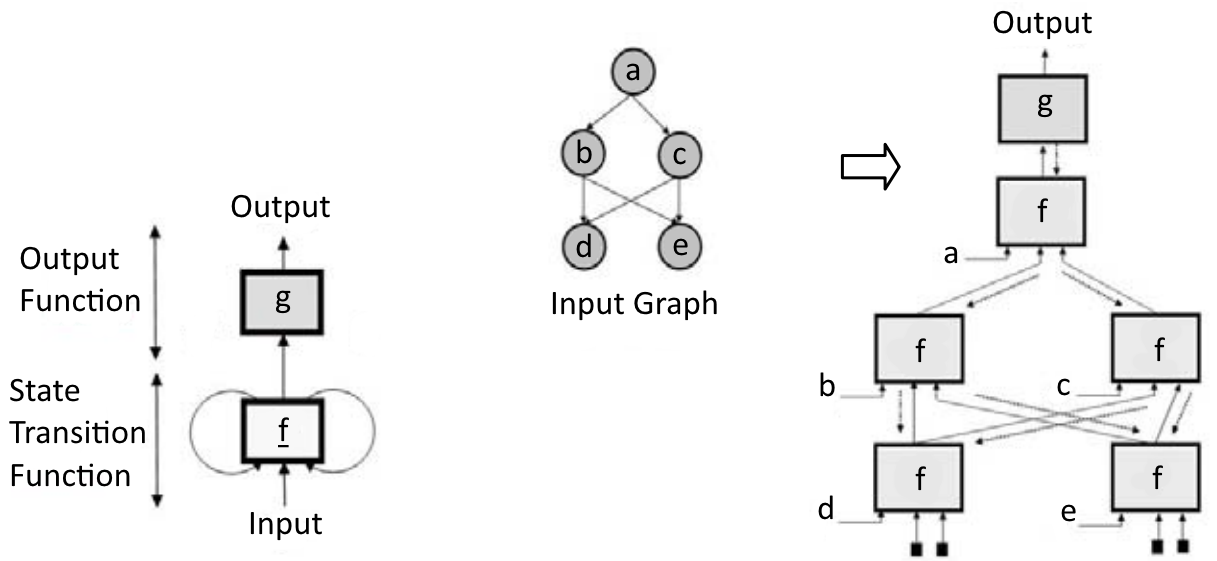
\includegraphics[height=7cm]{Fig1.png}
    \parbox[t][1.2cm][c]{16cm}{
        \centering
        Рис. 1. Пример входного графа и рекурсивной  нейронной сети
    }
\end{figure}


\subsection{Обучение}
Алгоритмы обучения нейронных сетей строятся на минимизации некоторой функции $E(W)$ - функции ошибки. Соответственно, изменяется ее параметр $W$.


В случае рекурсивных нейронных сетей фаза обучения состоит из подбора параметров функции изменения состояния $f$ и выходной функции $g$. Обозначим вектор параметров этих функций через $W = [w_1, w_2, \dots, w_m]$. Тогда возмущение функции ошибки относительно некоторой точки можно записать в виде\\ $E(W + \Delta W) = E(w_1 + \Delta w_1, w_2 + \Delta w_2, \dots, w_m + \Delta w_m)$. Воспользуемся разложением в ряд Тейлора этой функции:


\begin{multline}
\label{trivial}
E(W + \Delta W) = E(W) + \sum\limits_{i = 1}^m\frac{\partial E(W)}{\partial w_i}\Delta w_i +
\frac{1}{2}\sum\limits_{i = 1}^m\frac{\partial^2 E(W)}{\partial w_i^2}(\Delta w_i)^2 +\\
+\sum\limits_{i < j}\frac{\partial^2 E(W)}{\partial w_i \partial w_j}\Delta w_i \Delta w_j+
\frac{1}{6}\sum\limits_{i = 1}^m\frac{\partial^3 E(W)}{\partial w_i^3}(\Delta w_i)^3 + \dots
\end{multline}


Итак, каждое обновление параметров модели (весов) можно рассматривать как возмущение относительно некоторой точки, заданное $m$-мерным вектором. Пусть задана послудевательность из $N$ таких векторов с возмущением $\Delta W^i, i = \overline{1, N}$. В формуле $(3)$ отбросим все члены третьего и более высоких порядков и выразим математическое ожидание функции ошибки:


\begin{multline}
\label{trivial}
\mathbb{E}(E(W)) = \frac{1}{N}\sum\limits_{n = 1}^N E(W + \Delta W^n)\\
\mathbb{E}(E(W)) = E(W) + \sum\limits_{i = 1}^m\frac{\partial E(W)}{\partial w_i}\frac{1}{N}\sum\limits_{n=1}^N\Delta w_i^n+ \frac{1}{2}\sum\limits_{i=1}^m\frac{\partial^2E(W)}{\partial w_i^2}\frac{1}{N}\sum\limits_{n=1}^N(\Delta w_i^n)^2 
+\\+\sum\limits_{i<j}\frac{\partial^2E(W)}{\partial w_i\partial w_j}\frac{1}{N}\sum\limits_{n=1}{N}\Delta w_i^n\Delta w_j^n
\end{multline}


Перепишем равенство $(4)$ в терминах моментов случайных величин:


\begin{multline}
\mathbb{E}(E(W)) \cong E(W) + \sum\limits_{i=1}^m\mathbb{E}(\Delta w_i)\frac{\partial E(W)}{\partial w_i} +
\frac{1}{2}\sum\limits_{i=1}^{m}\mathbb{D}(\Delta w_i)\frac{\partial^2E(W)}{\partial w_i^2} +\\
+ \sum\limits_{i<j}cov(\Delta w_i, \Delta w_j)\frac{\partial^2E(W)}{\partial w_i \partial w_j}
\end{multline}


Так как обучение проводится методом градиентного спуска, то $\Delta w_i = -\eta g_i$.  Слагаемым, содержащим $cov(\Delta w_i, \Delta w_j)$, можно принебречь в предположении, что возмущенния не коррелируют в зависимости от $n$. $\mathbb{E}(\Delta w_i)\approx 0$, поэтому можно отбросить первую сумму в $(5)$. $\mathbb{D}(\Delta w_i)$ перепишем в виде $\sigma^2(\Delta w_i)$. В итоге получим:


\begin{equation}
\mathbb{E}(E(W)) \cong E(W) +
\frac{1}{2}\sum\limits_{i=1}^{m}\sigma^2(\Delta w_i)\frac{\partial^2E(W)}{\partial w_i^2} = E(W) + \frac{\eta^2}{2}\sum\limits_{i=1}^{m}\sigma^2(g_i)\frac{\partial^2E(W)}{\partial w_i^2}
\end{equation}


Видно, что значение ошибки достаточно сильно зависит от $\Delta w_i$. Поэтому, чтобы подавить возможный шум $\Delta w_i$ может быть заменено на $\eta g_i / \sigma(g_i)$. Заметим, что таким образом сигнал ошибки становится меньше, но в то же время меньше становится и объем информации, которую накапливает сеть. Это известная проблема, которая затрудняет поддержку долговременных связей. В случае рекурсивных нейросетей это становится особенно критично. Но с другой стороны, это позволяет избежать затухание градиента.


Таким образом обучение рекурсивной нейронной сети производится градиентным спуском второго порядка.
\section{Рекуррентные нейросети}

\subsection{Описание}
Рекуррентные нейронные сети - вид нейросетей, в которых связи между слоями образуют направленный цикл. Они являются частным случаем рекурсивной нейронной сети, с линейной структурой. Они так же используются для обработки последовательностей. Особенно часто для работы с рукописным текстом. Такие сети так же часто называются сетями Эльмана. Такие сети, в отличие от рекурсивных не позволяют учитывать иерархию обрабатываемых элементов, но распознают зависимость входной информации от порядка входа. Так же они отличаются довольно простой архитектурой.


Основная идея рекуррентной нейросети в том, чтобы помимо входного сигнала подавать на вход результат работы сети на предыдущем шаге. В первых реализациях на вместе со входным сигналом подавался выходной, но позже вместо него стали использовать результат работы скрытого слоя.



\subsection{Структура}
Для описания архитектуры рекуррентной нейронной сети рассмотрим двуслойный перцептрон. Копия вектора значений скрытого слоя отправляется в задержку (блок $D$ на рисунке 2). На каждом следующем шаге к входному сигналу добавляется сигнал, находящийся в задержке.

\begin{figure}[!h]
    \centering
        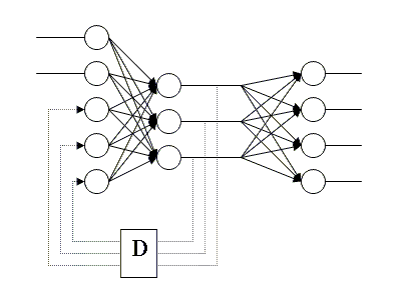
\includegraphics[height=7cm]{Fig2.png}
    \parbox[t][1.2cm][c]{16cm}{
        \centering
        Рис. 2. Рекурсивная нейросеть
    }
\end{figure}


В случае, если предыдущие результаты вносят слишком большой вклад, копия скрытого слоя, подающаяся на вход из задержки, домножается на коэффициент $W$.


\begin{figure}[!h]
    \centering
        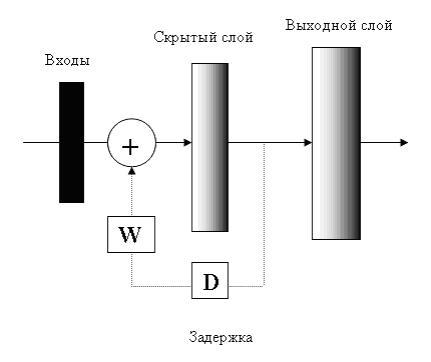
\includegraphics[height=7cm]{Fig4.jpg}
    \parbox[t][1.2cm][c]{16cm}{
        \centering
        Рис. 3. Использование коэффициента
    }
\end{figure}


В некоторых случаях, когда количество нейронов скрытого слоя равно количеству входов, на скрытый слой передают среднее арифметическое входного сигнала и вектора из задержки.
\subsection{Обучение}
Для обучения рекуррентных нейросетей используют алгоритм обратного распространения ошибки, который используется для многослойного перцептроа. Для обучения используются последовательности пар $(X_k^n, Y_k^n)$, где $k$ - номер последовательности, а $n$ - номер элемента в ней.


Выберем некоторую последовательность $(X_k, Y_k)$, с которой начнем обучение. В задержке выставляется нулевой вектор. Далее проведем коррекцию весов методом обратного распространения ошибки. Повторим коррекцию весов для оставшихся элементов последовательности учетывая задержку и заполняя её.


Далее следует повторять эту процедуру пока величина ошибки не станет достаточно мала.


Для обучения рекуррентных нейронных сетей используются различные алгоритмы оптимизации, например: имитация отжига или метод роя частиц.

\section{Long short term memory}

\subsection{Описание}
Long short term memory (LSTM, длительная кратковременная память) - вид рекуррентной нейронной сети, разработанный в 1997 году Юргеном Шмидхубером. LSTM, в отличие от простой рекуррентной нейросети, сохраняет связи между элементами с большим временным интервалом входа. Но в то же время данная архитектура не теряет связь между элементами последовательности с небольшим интервалом входа. Нейросети, которые были до этого, могли обрабатывать лишь небольшой диапозон интервалов, в основном небольшие интервалы.


Предшествующие архитектуры рекуррентных нейросетей имели проблемы в связи с алгоритмами обучения: backpropogation through time (BPTT) и real-time recurrent learning (RTRL). Основные проблемы связаны с одной стороны, с затуханием градиента и как следствие невозможность изменения некоторых весов и, с другой стороны, с нестабильностью весов, когда градиент имеет сильное влияние на изменение веса. LSTM использует константный поток ошибки, конкретнее Constant Error Carousel (CEC).


LSTM показывает более высокие результаты при распознавании рукописного текста или человеческой речи, чем обычные рекуррентные нейросети скрытые марковские модели. Именно этот вид нейронных сетей является наиболее популярным при распознавании речи.

\subsection{Constant Error Carousel}
Рассмотрим конкретнее подход CEC. Ожидаемый выходной сигнал для нейрона $k$ в момент времени $t$ обозначим $d_k(t)$. Запишем среднюю квадратичную ошибку для нейрона выходного слоя $k$:

\begin{equation}
\vartheta_k(t) = f_k'(net_k(t))(d_k(t) - y^k(t)),
\end{equation}


где
\begin{equation}
y^i(t) = f_i(net_i(t))
\end{equation}

- активация не входного нейрона $i$, а $f_i$ - дифференцируемая функция активации,


\begin{equation}
net_i(t) = \sum\limits_jw_{ij}y^j(t - 1)
\end{equation}

- сигнал, входящий в нейрон $i$, $w_{ij}$ - вес связи между нейронами $i$ и $j$.


Для нейронов не принадлежащих выходному слою:


\begin{equation}
\vartheta_j(t) = f_j'(net_j(t))\sum\limits_iw_{ij}\vartheta_i(t + 1).
\end{equation}


Таким образом, для отдельно взятого нейрона локольная ошибка в момент времени $t$ равна $\vartheta_j(t) = f_j'(net_j(t))\vartheta_j(t + 1)w_{jj}$. Для достижения константного потока ошибки необходимо выполнение равенства:

\begin{equation}
f_j'(net_j(t))w_{jj} = 1.0
\end{equation}


Проинтегрировав это равенство получим:

\begin{equation}
f_j(net_j(t)) = \frac{net_j(t)}{w_{jj}}
\end{equation}

Таким образом, функция $f_j$ должна быть линейной, а активация нейрона $j$ должна быть постоянной величиной:

\begin{equation}
y_j(t+1) = f_j(net_j(t+1)) = f_j(w_{jj}y_j(t)) = y_j(t)
\end{equation}

Этого можно добиться выбрав в качестве функции активации $f_j(x) \equiv x$ и выбрав в качестве веса $w_{jj} = 1.0$. Но нейрон, очевидно, имеет и другие, кроме связи ведущей в него же. В связи с этим появляются проблемы: конфликтов входящих весов и конфликт исходящих весов. Они сильно влияют только на обработку небольших интервалов, однако их эффект может распространиться и на большие интервалы.

\subsection{Структура}
Рассмотрим архитектуру LSTM. Для корректной работы нейрона, имеющего связь с самим собой (обозначим его $j$) и обеспечивающего CEC, вводятся два дополнительных элемента: шлюз входа (input gate unit) и шлюз выхода (output gate unit). Шлюз входа - мультипликативный нейрон, который осуществляет сохранность накопленных в $j$ данных от возмущений, связанных с некорректным вводом. Шлюз выхода - так же  мультипликативный нейрон, защищающий другие нейроны от шума, который находится в $j$.


Эти нейроны можно объединить в одну рабочую единицу, называемую клеткой памяти. Обозначим клетку памяти связанную с $j$ как $c_j$. Входные сигналы в $c_j$ состоят из трех сигналов: обычного входного сигнала сети $net_{c_j}$, выходного сигнала мультипликативного нейрона $out_j$ (от шлюза выхода) и выходного сигнала другого мультипликативного нейрона $in_j$ (от шлюза входа). Активацию последних двух обозначим как $y^{out_j}$ и $y^{in_j}$ соответственно.

\begin{figure}[!h]
    \centering
        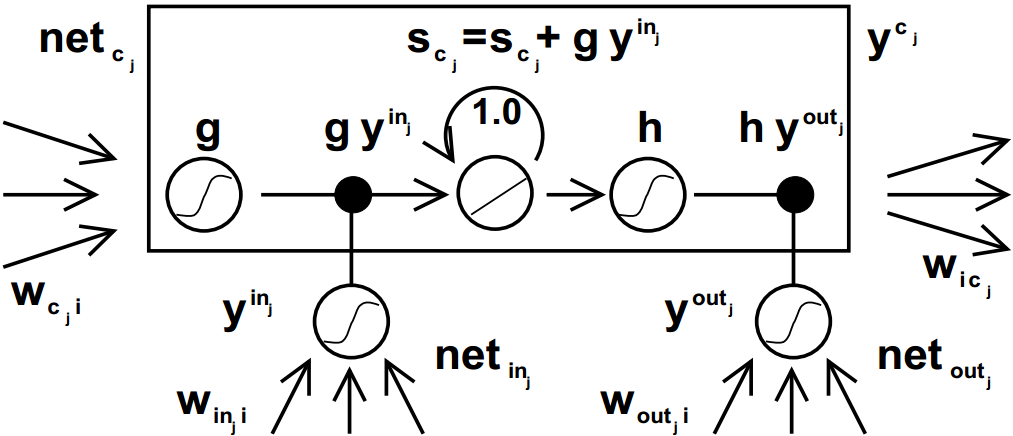
\includegraphics[height=7cm]{Fig3.png}
    \parbox[t][1.2cm][c]{16cm}{
        \centering
        Рис. 4. Модель клетки памяти
    }
\end{figure}


\begin{equation}
y^{out_j}(t) = f_{out_j}(net_{out_j}(t)); y^{in_j}(t) = f_{in_j}(net_{in_j}(t));
\end{equation}

где

\begin{eqnarray}
net_{out_j}(t) = \sum\limits_uw_{out_ju}y^u(t - 1),\nonumber\\
net_{in_j}(t) = \sum\limits_uw_{in_ju}y^u(t - 1),\nonumber
\end{eqnarray}


Так же мы имеем
\begin{eqnarray}
net_{с_j}(t) = \sum\limits_uw_{с_ju}y^u(t - 1),\nonumber
\end{eqnarray}

Суммирование ведется по элементам всех видов: клетки памяти, входные нейроны, шлюзовые нейроны и возможно скрытые нейроны (если их наличие соответствует архитектуре).  Шлюзовые нейроны могут получать на вход сигналы от других клеток памяти, для того, чтобы контроллировать информацию поступающую в клетку памяти. Так же могут быть рекуррентные клетки памяти.

\begin{figure}[!h]
    \centering
        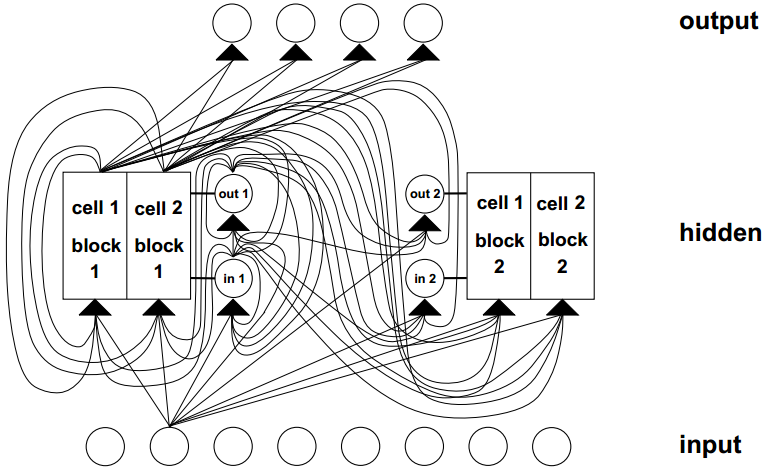
\includegraphics[height=9cm]{Fig5.png}
    \parbox[t][1.2cm][c]{16cm}{
        \centering
        Рис. 5. Пример сети LSTM
    }
\end{figure}


Во момент времени $t$ выходной сигнал клетки $c_j$ вычислсяется следующим образом:

\begin{equation}
y^{c_j}(t) = y^{out_j}(t)h(s_{c_j}(t)),\nonumber
\end{equation}

где $s_{c_j}(t)$ - внутреннее состояние клетки $c_j$ в момент времени $t$.

\begin{equation}
s_{c_j}(0) = 0,~s_{c_j}(t) = s_{c_j}(t - 1) + y^{in_j}(t)g(net_{c_j}(t)),\nonumber
\end{equation}

Функции $g$ и $h$ масштабируют соответственно входной и выходной сигналы клетки памяти.


Шлюзы используются, чтобы предотвратить конфликт входного сигнала  и конфликт выходного сигнала. Сеть использует их чтобы решить какую информацию можно передать клетке и каую информацию может передать клетка. Так как в этой модели используется CEC, то ошибка остается внутри клетки, но со временем ошибка, содержащаяся во входном сигнале может уменьшить текущую ошибку.


Клетку памяти можно объединять в блоки и работать с блоками, как с отдельными элементами.

\subsection{Обучение}
Для обучения сети LSTM используется градинтный спуск, если конкретнее метод обратного распространения ошибки во времени (BPTT). Оснвная проблема этого метода для рекуррентных сетей - это затухание градиента, но так как в LSTM используется Constant Error Carousel, то этой проблемы нет.


LSTM так же может быть обучен путем комбинирования эволюционных алгоритмов для весов скрытого слоя и метода опорных векторов для весов выходного слоя. При обучении с подкреплением используются методы эволюционных стратегий или генетические алгоритмы.


\section{Примеры использования рекурсивных сетей}

\subsection{Обработка естественных языков}
Для обработки естественных языков удобно использовать глубокие нейронные сети. В таких сетях каждый новый слой представляет новый уровень абстракции и переводит вектор значений предыдущего слоя в вектоор меньшей размерности.


Используемые для этих целей рекурсивные нейронные сети имеют древовидную структуру. Каждый новый уровень узлов в таком дереве представляет новый уровень абстракции и содержит информацию от двух узлов предыдущего уровня. Таким образом в корне содержится вектор, содержащий необходимую информацию о обработанном тексте.
Именно значение в корне и является результатом работы сети и используется для классификации текста или каких-либо других задач.


Так же для обработки текста может использоваться рекуррентная сеть. В этом случае текст передается на вход отдельными словами, как последовательность. Соответственно принцип работы рекуррентной нейронной сети несколько отличается от рекурсивной.
\pagebreak
\begin{figure}[!h]
    \centering
        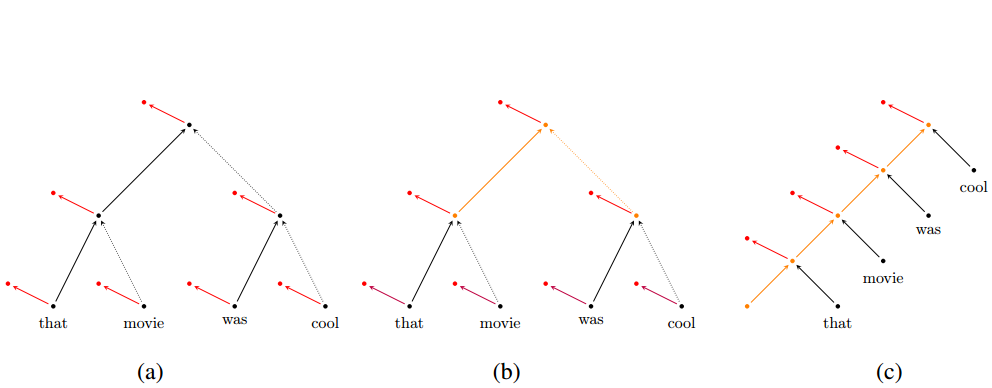
\includegraphics[width=16cm]{Fig6.png}
    \parbox[t][1.2cm][c]{16cm}{
        \centering
        Рис. 6. Примеры рекурсивной сети (a, b) и рекуррентной (c)
    }
\end{figure}


Глубина рекурсивной сети при таком подходе ограничена максимальным количеством слов, подаующихся на вход. Поэтому можно использовать глубокие рекурсивные нейронные сети, полученные путем соединения нескольких слоев рекурсивных нейронных сетей. Таким образом, мы можем увеличить уровень абстракции информации, с которой работаем.


Рассмотрим принцип работы такой сети более детально. Для начала обратим внимание на структуру простого слоя в глубокой сети. Это бинарное дерево, в листья которого передаются векторные представления слов. Представление каждого внутреннего узла $\eta$ выражается следующим образом:


\begin{equation}
x_\eta=f(W_Lx_{l(\eta)} + W_Rx_{r(\eta)} + b),
\end{equation}


где $l(\eta)$ и $r(\eta)$ - левый и правый дети узла $\eta$ соответственно. $W_L$ и $W_R$ - матрицы весов, а $b$ - вектор смещения. Иногда эту формулу представляют в другом виде:


\begin{equation}
x_\eta=f(Wx_{l, r} + b),
\end{equation}

где $x_{l, r}$ вектор составленный из векторов $x_l(\eta)$ и $x_r(\eta)$, а матрица $W$ - является матрицей, составленной из $W_L$ и $W_R$.


Заметим, что матрицы $W_L$ и $W_R$ - квадратные. То есть, промежуточные узлы переводят вектора из некоторого простарнства в него же. Это можно интерпретировать, как объединение смысла исходных подфраз.


Для узлов выходного слоя так же должна быть определена функция, формирующая выходной сигнал:

\begin{equation}
y_\eta=g(Ux_\eta + c),
\end{equation}

где $y_\eta$ - выходной сигнал, $U$ - матрица весов выхода, а $c$ - вектор смещения. При обучении нейросети с учителем - именно $y_\eta$ используется в качестве ответа сети.


Можно условно разделить формулу $(15)$ на формулу для листьев и на формулу для внутренних узлов. Пусть внутренние узлы работают в некотором пространстве $\mathcal{H}$, а входной сигнал принадлежит пространству $\mathcal{X}$. Тогда в общем виде формула $(15)$ будет выглядеть так:


\begin{equation}
h_\eta=f(W_L^{l(\eta)}h_{l(\eta)} + W_R^{r(\eta)}h_{r(\eta)} + b),
\end{equation}


где $h_\eta = x_\eta \in \mathcal{X}$ для листа и $h_\eta \in \mathcal{H}$ для остальных узлов. $W^\eta = W^{xh}$, если $\eta$ - лист и $W^\eta=W^{hh}$ иначе.


Теперь рассмотрим конечный вариант такой архитектуры, то есть глубокую рекурсивную нейросеть. Как уже говорилось выше, мы получаем ее накладывая слои друг на друга и тем самым добиваемся большего уровня абстракции. При этом формулы так же изменят вид:

\begin{equation}
h_\eta^{(i)}=f(W_L^{(i)}h_{l(\eta)}^{(i)} + W_R^{(i)}h_{r(\eta)}^{(i)} + V^{(i)}h_\eta^{(i - 1)} + b^{(i)}),
\end{equation}

где $i$ - номер слоя.

\begin{figure}[!h]
    \centering
        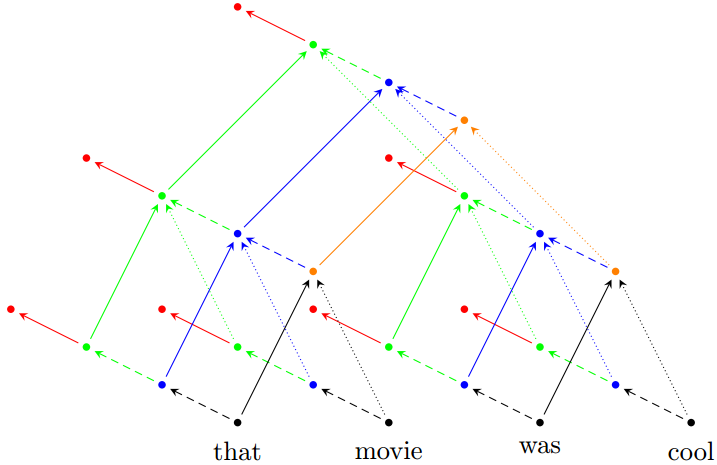
\includegraphics[width=16cm]{Fig7.png}
    \parbox[t][1.2cm][c]{16cm}{
        \centering
        Рис. 7. Глубокая рекурсивная нейронная сеть
    }
\end{figure}

Формула для выходного сигнала примет вид:

\begin{equation}
y_\eta=g(Uh_\eta^{(l)} + c),
\end{equation}


где $l$ - количество слоев.


Рекурсивные нейросети широко используются для обработки текстов, так как сохраняют связи слов. Напаример, группа ученых из Стенфорда создала нейронную сеть на основе такой архитектуры, способную определять тональность фразы с точностью $85\%$, что является удивительным результатом, так как не все люди способны на это.

\begin{figure}[!h]
    \centering
        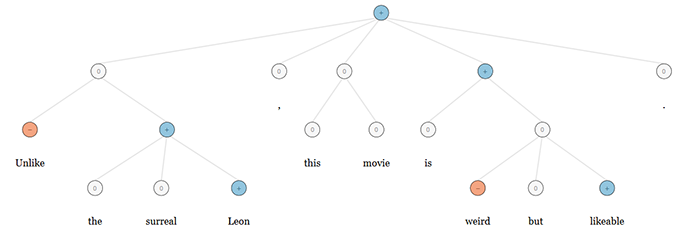
\includegraphics[width=16cm]{Fig8.png}
    \parbox[t][1.2cm][c]{16cm}{
        \centering
        Рис. 9. Сравнение деревьев и матриц для изображения и текста
    }
\end{figure}

\subsection{Обработка изображений}
Рекурсивные структуры повсеместно встречаются в изображениях. Так например мы можем выделить на фотографии некоторые объекты, разбить каждый из них на подъобъекты и так далее. Поэтому для анализа изображений можно применять рекурсивные нейронные сети.

Начав сливать части изображения мы, во-первых, получаем все изображение, во-вторых, получаем дерево, которое описывает весь процесс слияния. Так как, в отличие от текста, объект на изображении может быть связан с более чем двумя другими объектами, то для одной и той же картинки можно получить различные деревья слияния. Для получения таких деревьев применяют жадные алгоритмы, которые выбирают очередное слияние путем максимизации некоторой метрики.


Так же, для объектов на изображении можно составить матрицу, в которой значение элемента $(i, j)$ будет показываеть наличие или отсутствие связи между объектами с номерами $i$ и $j$.

\begin{figure}[!h]
    \centering
        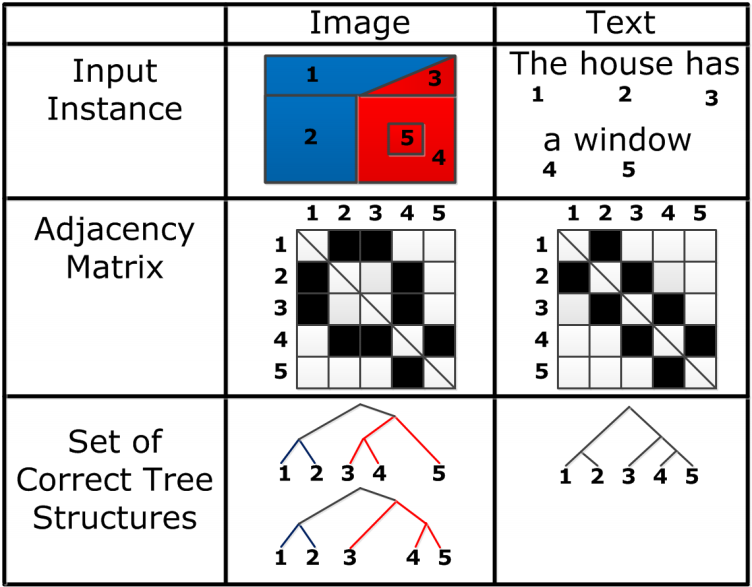
\includegraphics[width=14cm]{Fig9.png}
    \parbox[t][1.2cm][c]{16cm}{
        \centering
        Рис. 8. Дерево, определяющее тональность фразы
    }
\end{figure}


Как мы видим, работа с рекурсивными нейросетями для обработки изображений имеет много общего с рекурсивными сетями, специализирующимися на работе с текстом. В итоге такие нейросети способны самостоятельно выделять объекты на изображении и классифицировать их.


\pagebreak

\section{Заключение}
Рекурсивные нейронные сети имеют практическую значимость благодаря тому, что сохраняют связи между объектами с которыми производится работа. Наиболее популярно их использование при обработке текстов и изображений, то есть в тех областях, где нельзя обрабатывать какую либо часть данных отдельно от всего контекста.


Рекуррентные нейронные сети имеют, как правило, несколько более просту структуру. Они удобны для обработки потока информации.


Так же стоит отдельно выделить Long Short Term Memory. Этот вид рекуррентных нейросетей показывает хороший результат при обработке речи, так как благодаря своей архитектуре сохраняет информацию о предыдущих сигналах на протяжении длительного времени.


\pagebreak


\LARGE\bibname

\large
1. Parsing Natural Scanes and Natural Language with Recursive Neural Network / Richard Socher и др. // Computer Science Departament, Stanford University, Stanford


2. Ozan Irsoy. Deep Recursive Neural Networks for Compositionality in Language / Ozan Irsoy, Claire Cardie


3. Alejandro Chinea. Underatanding the Principles of Recursive Neural Networks: A Generative Approach to Tackle Model Complexity / Alejandro Chinea


4. Jürgen Schmidhuber. Long Short-Term Memory / Jürgen Schmidhuber // Neural Computation. - 1997 - №9(8)


5. Recursive Neural Network. - https://en.wikipedia.org/wiki/Recursive\_neural\_network


6. Recurrent Neural Network. - https://en.wikipedia.org/wiki/Recurrent\_neural\_network


7. LSTM. - https://en.wikipedia.org/wiki/Long\_short\_term\_memory


8. Популярные нейросетевые архитектуры. - http://cgm.computergraphics.ru/content/view/57
\end{document}
